\documentclass[]{article}
\usepackage[spanish.mexico]{babel}
\usepackage[T1]{fontenc}
\usepackage[utf8]{inputenc}
%\usepackage{lmodern}
\usepackage[a4paper]{geometry}

%Graficos e imagenes
\usepackage{graphicx}
\usepackage{subcaption}

%multicolumna
\usepackage{multicol}

\usepackage{cite}

%Grafico de barras
%\usepackage{pgfplots}




%\title{Proyecto de Optimización de Energía}
%\author{Pablo Vivar Colina}
%\date{Mayo 2018}



\begin{document}
	
%\usepackage[top=2cm,bottom=2cm,left=1cm,right=1cm]{geometry}


\begin{titlepage}
     \begin{center}
	
\includegraphics[width=0.09\textwidth]{UNAM}\Large Universidad Nacional Autónoma de México
        	
\includegraphics[width=0.09\textwidth]{FI}\\[1cm]
        \Large Facultad de Ingeniería\\[1cm]
       % \Large División de Ciencias Básicas\\[1cm]
         \Large Laboratorio de Fundamentos de Control(6655)\\[1cm]
         %la clave antes era:4314
         \footnotesize Profesor: Salcedo Ubilla María Leonor Ing.\\[1cm]
        \footnotesize Semestre 2019-1\\[1cm]
        
       

        \Large Práctica No. 1\\[1cm]
        
           

\Large Introdcción MATLAB
        
         %Texto a la derecha
          \begin{flushright}
\footnotesize  Grupo 2\\[0.5cm]
\footnotesize Brigada: 4\\[0.5cm]
\footnotesize Rodrigo Adrián Martínez López\\[0.5cm]
\footnotesize Vivar Colina Pablo\\[0.5cm]
 \end{flushright}
    %Texto a la izquierda
          \begin{flushleft}
        \footnotesize Ciudad Universitaria Agosto de 2018.\\
          \end{flushleft}
         
          
        %\vfill
        %\today
   \end{center}
\end{titlepage}
 %agregar portada

%\maketitle

\tableofcontents  % Write out the Table of Contents

%\listoffigures  % Write out the List of Figures

\section{Resumen}

\section{Introducción}



\subsection{NI ELVIS}

Para crear una aplicación completa de NI ELVIS, explore otras soluciones de laboratorio para NI ELVIS.\\

Proporciona una experiencia de aprendizaje basada en proyectos, usando medidas en línea y diseño práctico y embebido.\\

El NI Educational Laboratory Virtual Instrumentation Suite (NI ELVIS) es un dispositivo modular de laboratorio educativo de ingeniería desarrollado específicamente para la academia. Con este enfoque práctico, los profesores pueden ayudar a los estudiantes a aprender habilidades de ingeniería prácticas y experimentales. NI ELVIS incluye un osciloscopio, multímetro digital, generador de funciones, fuente de alimentación variable, analizador de Bode y otros instrumentos comunes de laboratorio. Puede conectar una PC al NI ELVIS usando USB y desarrollar circuitos en su protoboard desmontable.\cite{NationalInstruments2018}\\

\section{Objetivos}


	\begin{itemize}
		\item Utilizar la herramientas de National Instruments para verificar las ecuaciones de función de transferencia
	\end{itemize}



\section{Materiales y métodos}

	\begin{itemize}
		\item NI Elvis
		\item Computadora con Suite de herramientas Texas Instruments
	\end{itemize}
	
\section{Resultados}



Se usa el circuito operacional (741) con realimentacion negativa.\\


\begin{itemize}

	\item 2->Entrada Inversora
	\item 3->Entrada no inversora
	\item 4->Fuente -10[V]
	\item 5->Vacío
	\item 6->Salida
	\item 7->Fuente +10[V]
\end{itemize}


$i_1$ es la corriente que entra en la resistencia 1 a pin inversor 741
$i_2$ es la corriente de la resistencia 2 que va entre los pines 2 y 6.\\

\begin{multicols}{2}

\begin{equation}
   i_1+i_2=0
\end{equation}

\begin{equation}
    i_1=\frac{V_e-V_a}{R_1}
\end{equation}

\begin{equation}
   i_2=\frac{V_s-V_a}{R_2}
\end{equation}

\begin{equation}
    V_b=0
\end{equation}

\begin{equation}
    V_b=V_a
\end{equation}

\begin{equation}
    V_a=0
\end{equation}

\begin{equation}
    \frac{V_e}{R_1}+\frac{V_s}{R_2}=0
\end{equation}

\begin{equation}
   \frac{V_s}{V_e}=-\frac{R_2}{R_1}
\end{equation}

\end{multicols}

Ganancia del circuito


\begin{figure}[h!]
	\centering
	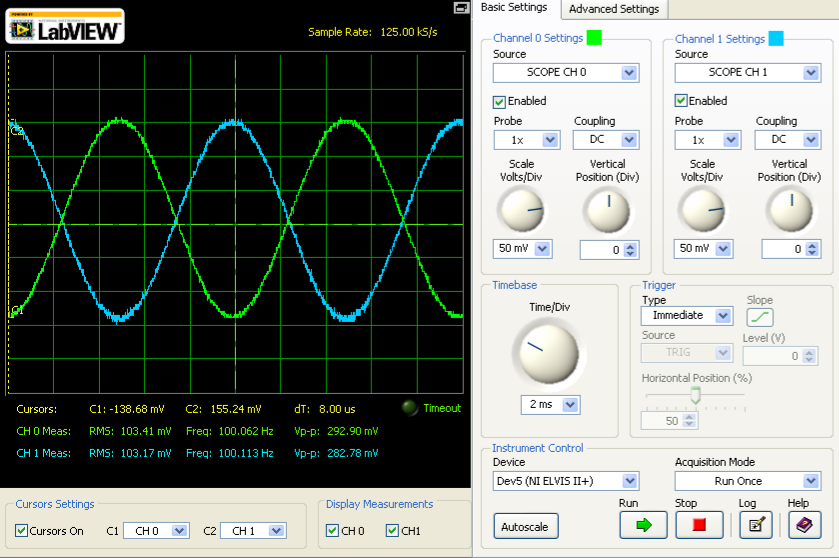
\includegraphics[width=0.6\textwidth]{Imagenes/primerCircuito.png}
	\caption{Respuesta de primer circuito}
	\label{fig:primerCircuito}
\end{figure}

En el la gráfica que se presenta en la figura \ref{fig:primerCircuito} en la cuál se puede observar el correcto funcionamiento de la entrada inversora del amplificador operacional.\\



\begin{figure}[h!]
	\centering
	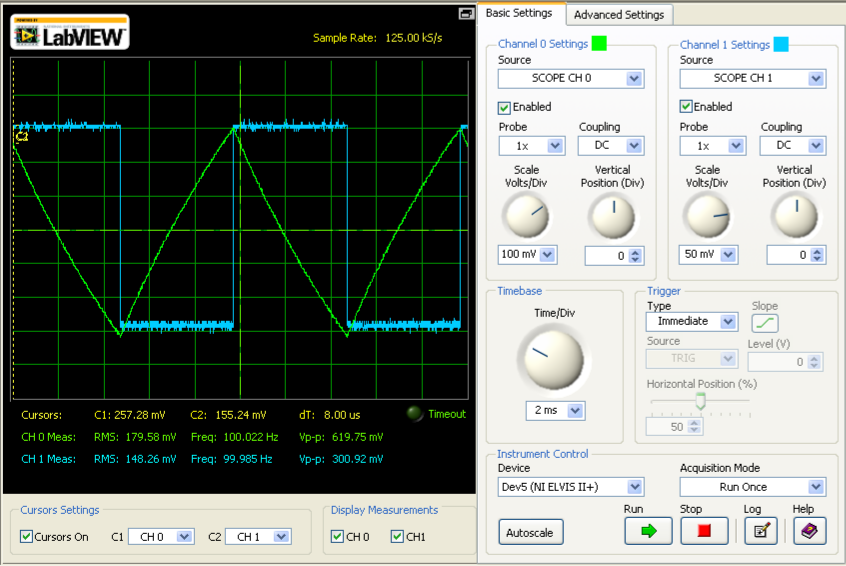
\includegraphics[width=0.6\textwidth]{Imagenes/circuito3.png}
	\caption{Señales de entrada y salida en el Circuito 3 (integrador)}
	\label{fig:circuito3}
\end{figure}

En la figura \ref{fig:circuito3} logramos ver el comportamiento del amplificador operacional como integrador


% PRIMER BLOQUE DE 3 IMAGENES
\begin{figure}[h!]
	
	\centering
	\begin{subfigure}[b]{0.45\textwidth}
		
		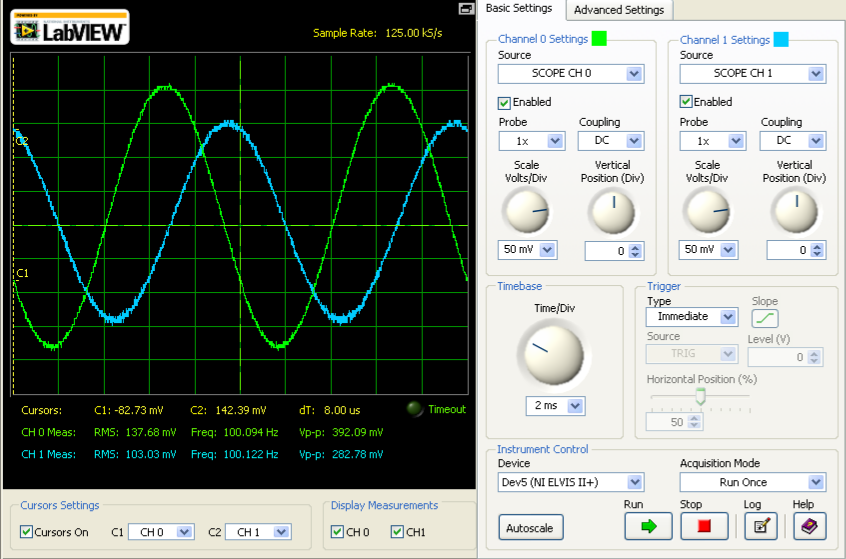
\includegraphics[width=\textwidth]{Imagenes/circuito3Senoidal.png}
		\caption{Señal Senoidal}
		\label{fig:circuito3Senoidal}
		
	\end{subfigure}
	~ 
	\begin{subfigure}[b]{0.45\textwidth}
	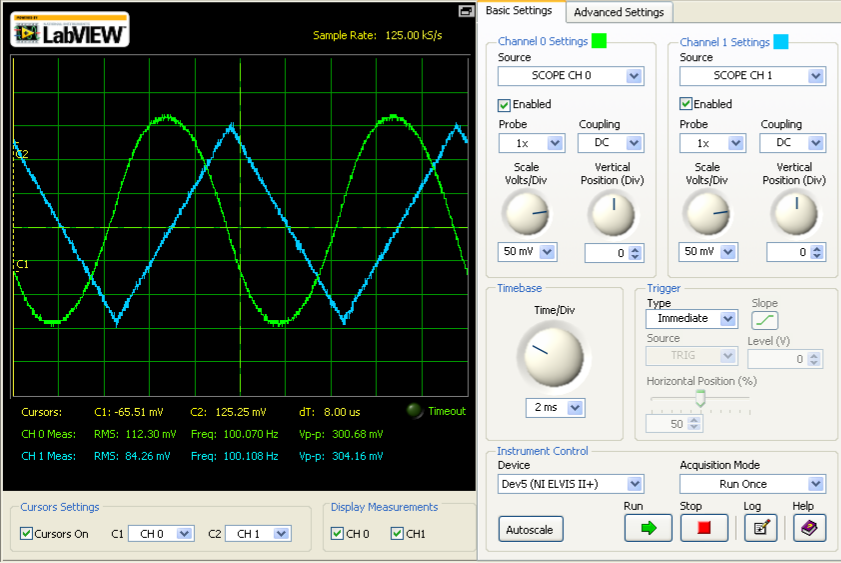
\includegraphics[width=\textwidth]{Imagenes/circuito3Triangular.png}
	\caption{Señal Triangular}
	\label{fig:circuito3triangular}	
	
	\end{subfigure}
	~ 
	\begin{subfigure}[b]{0.45\textwidth}
		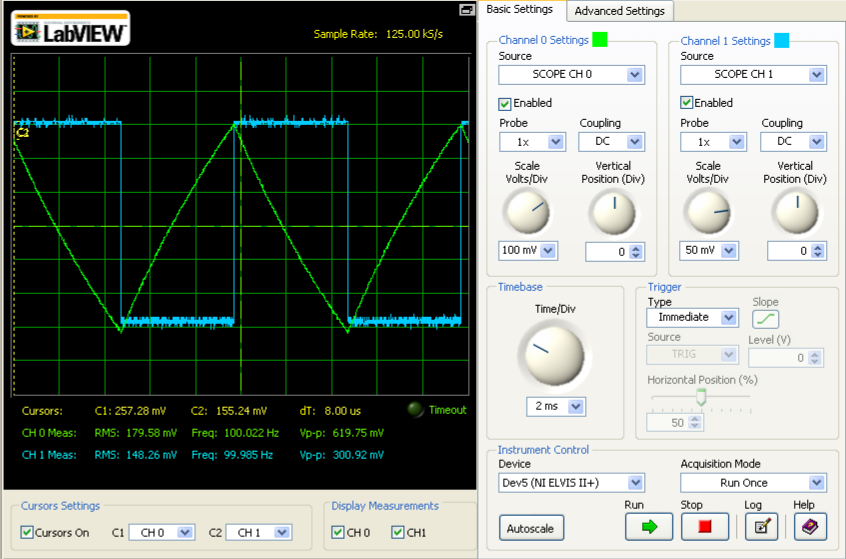
\includegraphics[width=\textwidth]{Imagenes/circuito3Cuadrada.png}
		\caption{Señal Cuadrada}
		\label{fig:circuito3cuadrada}
	\end{subfigure}
	
	\caption{Señales de entrada y de salida del circuito 3}\label{fig:circuito3Signals}
	
\end{figure}

Así como en la figura \ref{fig:circuito3}, en la figura \ref{fig:circuito3Signals} logramos ver el comportamiento del circuito 3, con las señales de entrada senoidal, cuadrada y triangular.\\

% Segundo BLOQUE DE 3 IMAGENES
\begin{figure}[h!]
	
	\centering
	\begin{subfigure}[b]{0.45\textwidth}
	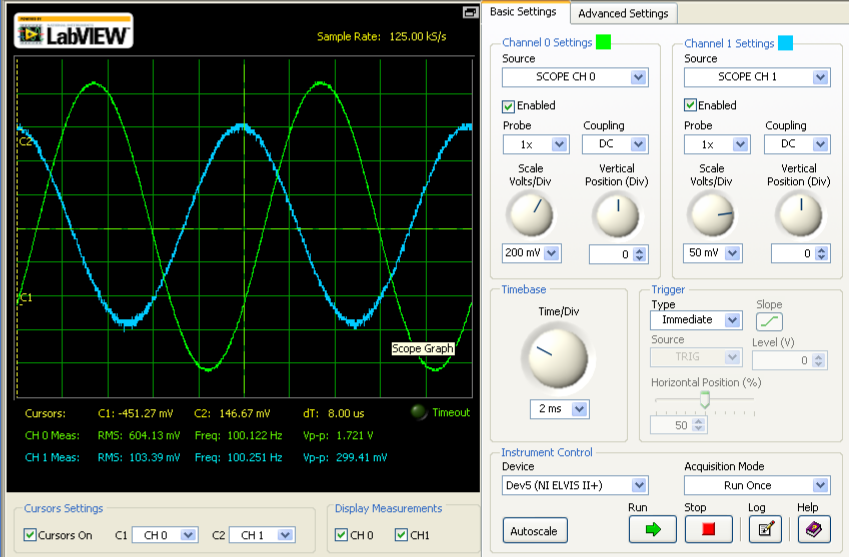
\includegraphics[width=\textwidth]{Imagenes/circuito4senoidal.png}
	\caption{Señal Senoidal}
	\label{fig:circuito4seonidal}
\end{subfigure}
~ 
\begin{subfigure}[b]{0.45\textwidth}
	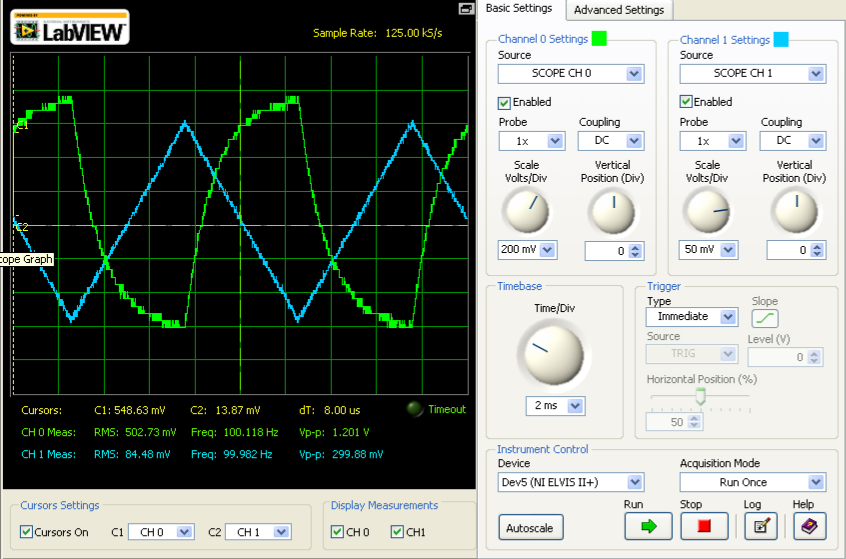
\includegraphics[width=\textwidth]{Imagenes/circuito4triangular.png}
	\caption{Señal Triangular}
	\label{fig:circuito4triangular}
\end{subfigure}
~ 
\begin{subfigure}[b]{0.45\textwidth}
	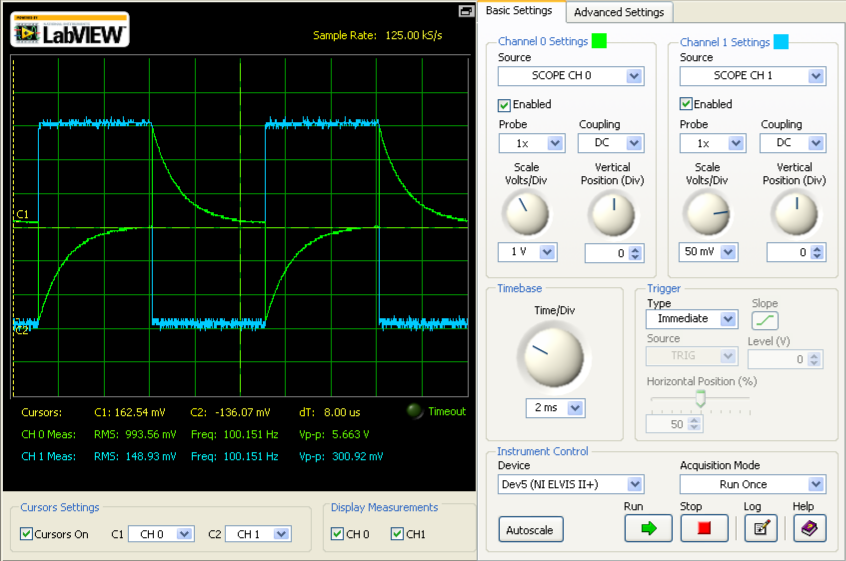
\includegraphics[width=\textwidth]{Imagenes/circuito4cuadrada.png}
	\caption{Señal Cuadrada}
	\label{fig:circuito4cuadrada}
\end{subfigure}
	\caption{Señales de entrada y de salida del circuito 4}\label{fig:circuito4Signals}
	
\end{figure}

En la figura \ref{fig:circuito4Signals} logramos ver el comportamiento del circuito 4, con las señales de entrada senoidal, cuadrada y triangular.\\

\begin{figure}[h!]
	\centering
	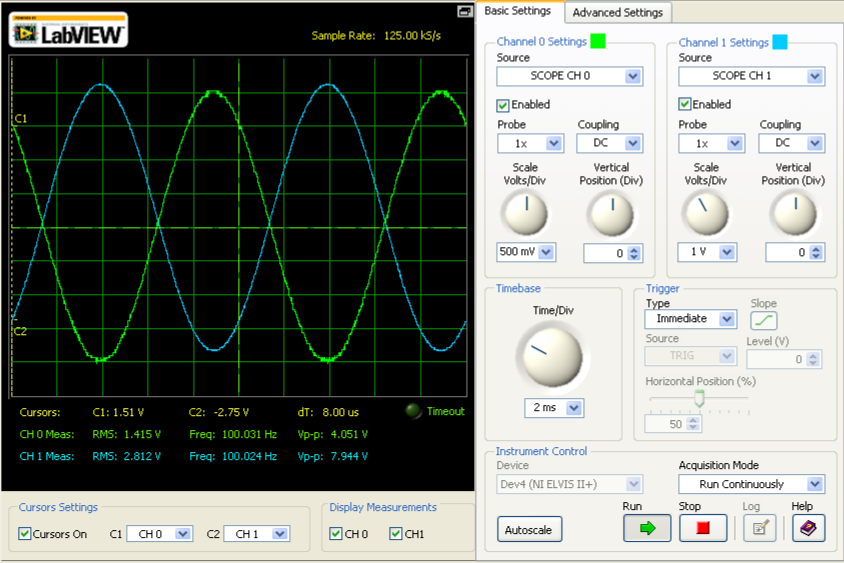
\includegraphics[width=0.5\textwidth]{Imagenes/circuito5sumador.png}
	\caption{Circuito Sumador}
	\label{fig:circuito5sumador}
\end{figure}

En la figura \ref{fig:circuito5sumador} se puede apreciar el comportamiento en la entrada y salida del circuito Sumador\\

% Tercer BLOQUE DE 3 IMAGENES
\begin{figure}[h!]
	
	\centering
	\begin{subfigure}[b]{0.45\textwidth}
		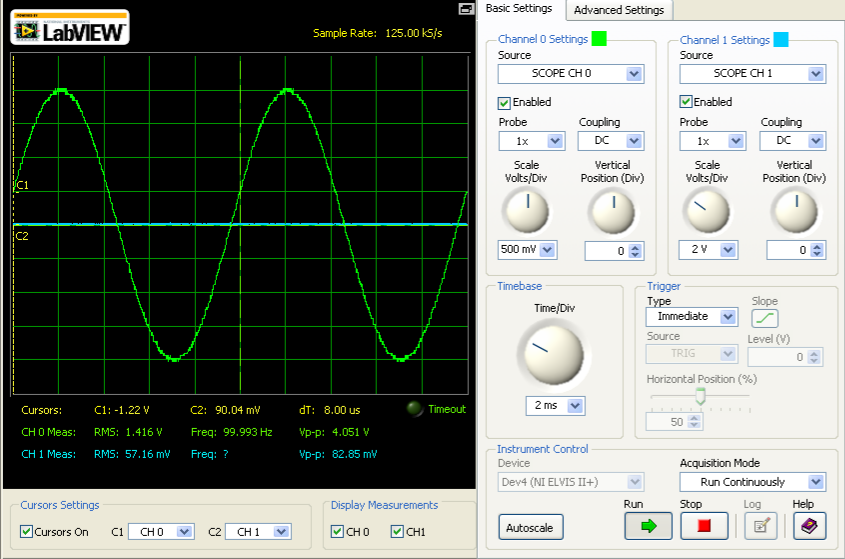
\includegraphics[width=\textwidth]{Imagenes/circuito5generadorVA.png}
		\caption{Generador de funciones en terminal A}
		\label{fig:circuito5generadorVA}
	\end{subfigure}
	~ 
	\begin{subfigure}[b]{0.45\textwidth}
		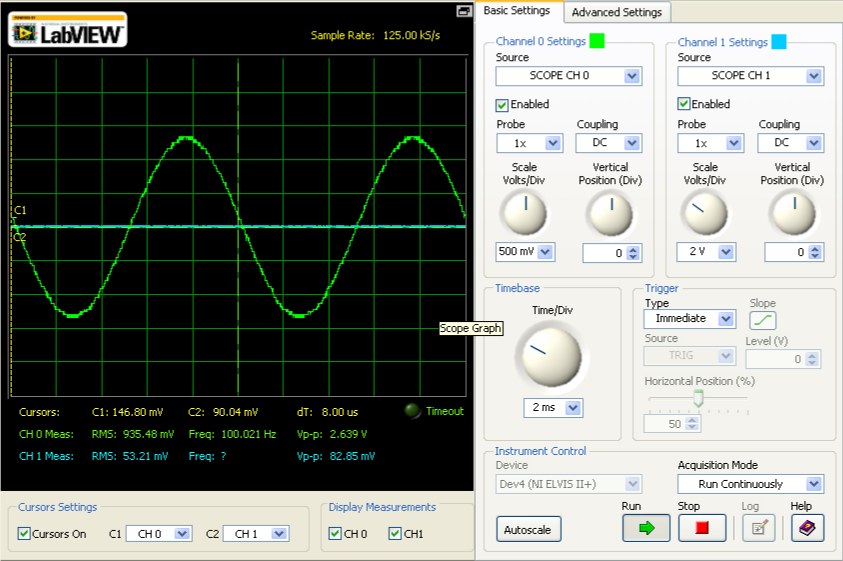
\includegraphics[width=\textwidth]{Imagenes/circuito5generadorVB.png}
		\caption{Generador de funciones en terminal B}
		\label{fig:circuito5generadorVB}
	\end{subfigure}
	~ 
	\begin{subfigure}[b]{0.45\textwidth}
		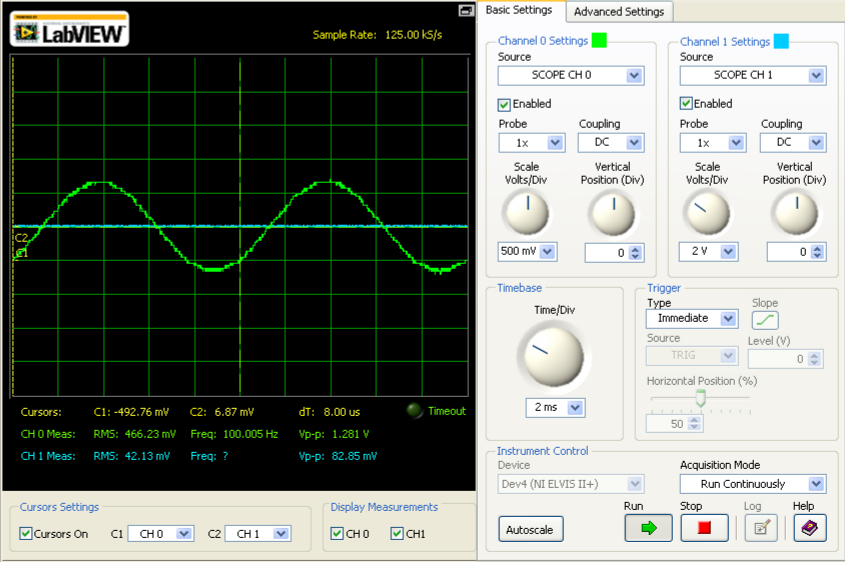
\includegraphics[width=\textwidth]{Imagenes/circuito5generadorVC.png}
		\caption{Generador de funciones en terminal C}
		\label{fig:circuito5generadorVC}
	\end{subfigure}
	\caption{Señales de entrada al circuito 5}\label{fig:circuito5InputSignals}
	
\end{figure}

% Cuarto  BLOQUE DE 3 IMAGENES
\begin{figure}[h!]
	
	\centering
	\begin{subfigure}[b]{0.45\textwidth}
		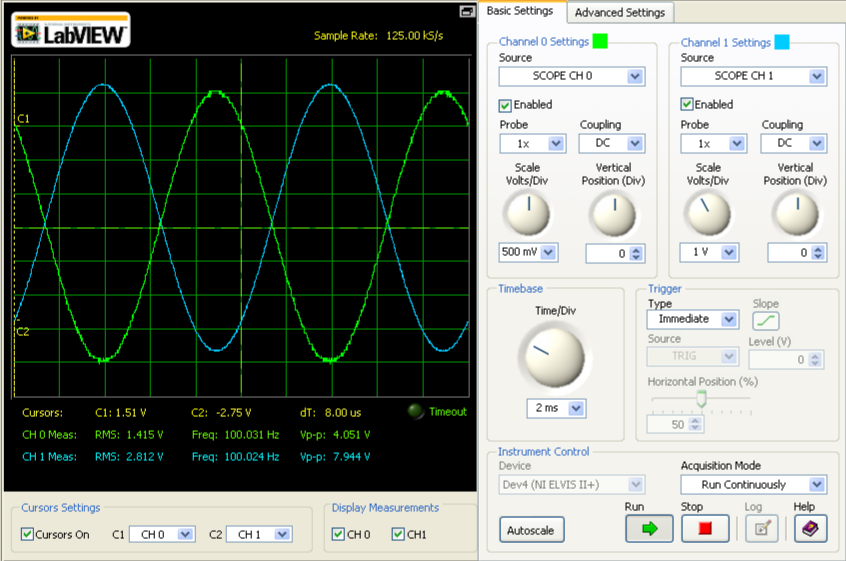
\includegraphics[width=\textwidth]{Imagenes/circuito5sumadorVA.png}
		\caption{Sumador en Terminal A}
		\label{fig:circuito5sumadorVA}
	\end{subfigure}
	~ 
	\begin{subfigure}[b]{0.45\textwidth}
		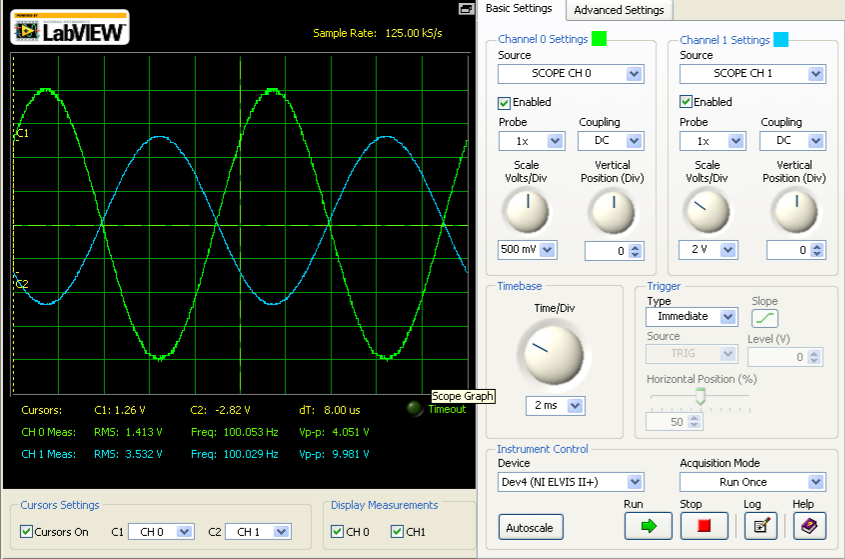
\includegraphics[width=\textwidth]{Imagenes/circuito5sumadorVB.png}
		\caption{Sumador en Terminal B}
		\label{fig:circuito5sumadorVB}
	\end{subfigure}
	~ 
	\begin{subfigure}[b]{0.45\textwidth}
		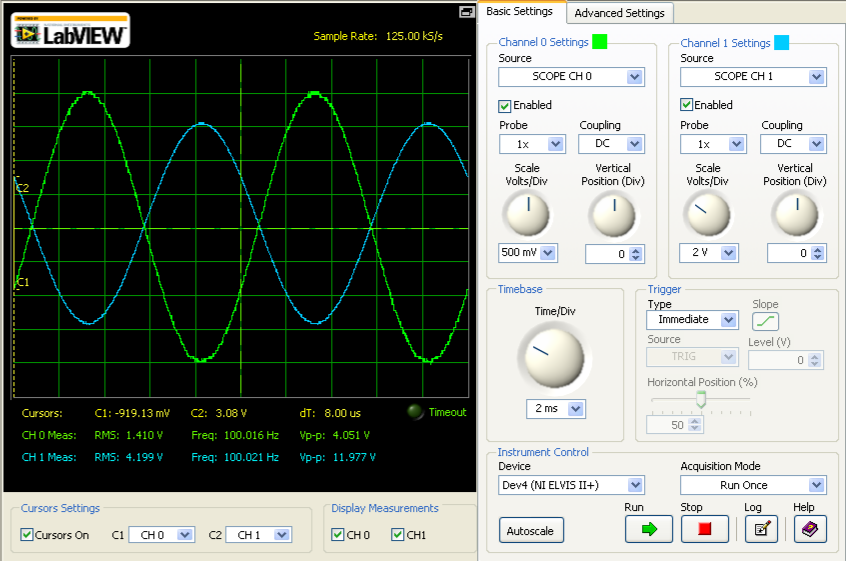
\includegraphics[width=\textwidth]{Imagenes/circuito5sumadorVC.png}
		\caption{Sumador en Terminal C}
		\label{fig:circuito5sumadorVC}
	\end{subfigure}
	\caption{Señales de salida del circuito 5 (sumador)}\label{fig:circuitoSumadorOutput}
	
\end{figure}

% Quinto  BLOQUE DE 3 IMAGENES
\begin{figure}[h!]
	
	\centering
	\begin{subfigure}[b]{0.45\textwidth}
		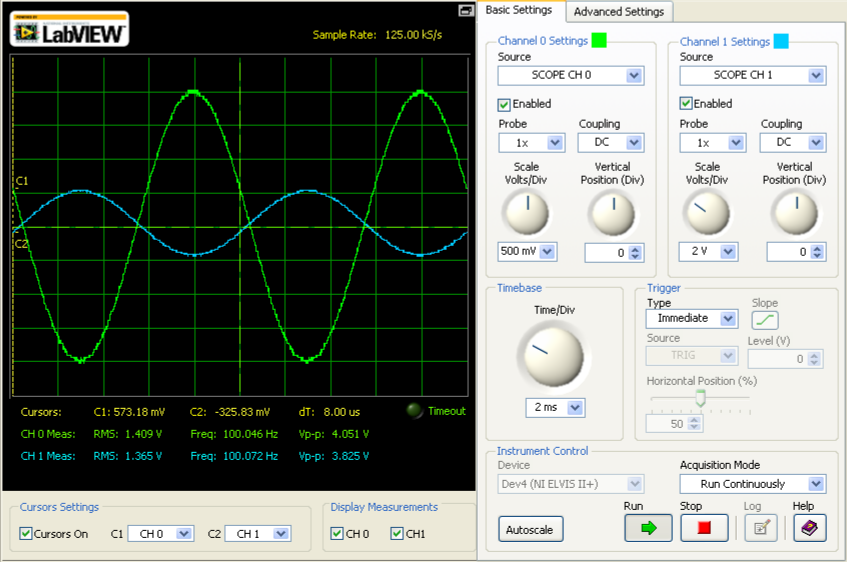
\includegraphics[width=\textwidth]{Imagenes/VAmasVB.png}
		\caption{Sumador en Terminales A y B}
		\label{fig:VAmasVB}
	\end{subfigure}
	~ 
	\begin{subfigure}[b]{0.45\textwidth}
		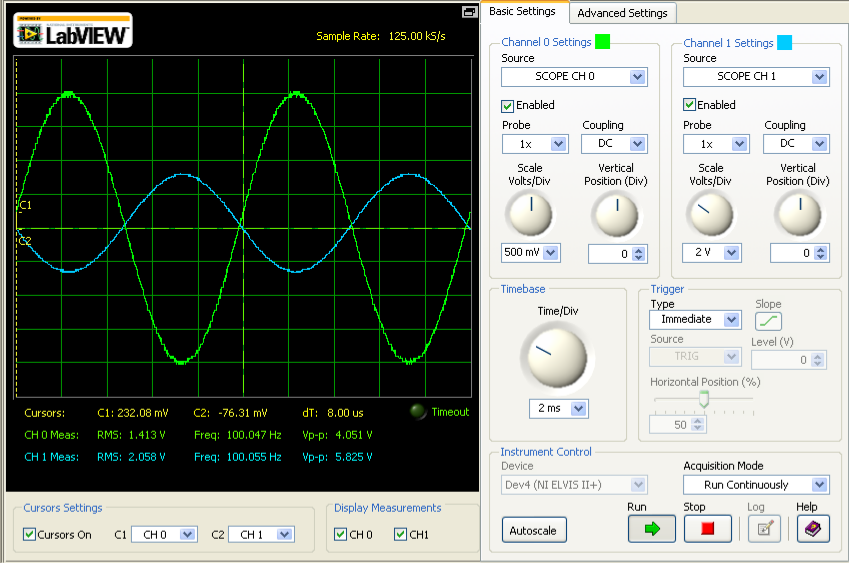
\includegraphics[width=\textwidth]{Imagenes/VAmasVC.png}
		\caption{Sumador en Terminales A y C}
		\label{fig:VAmasVC}
	\end{subfigure}
	~ 
	\begin{subfigure}[b]{0.45\textwidth}
		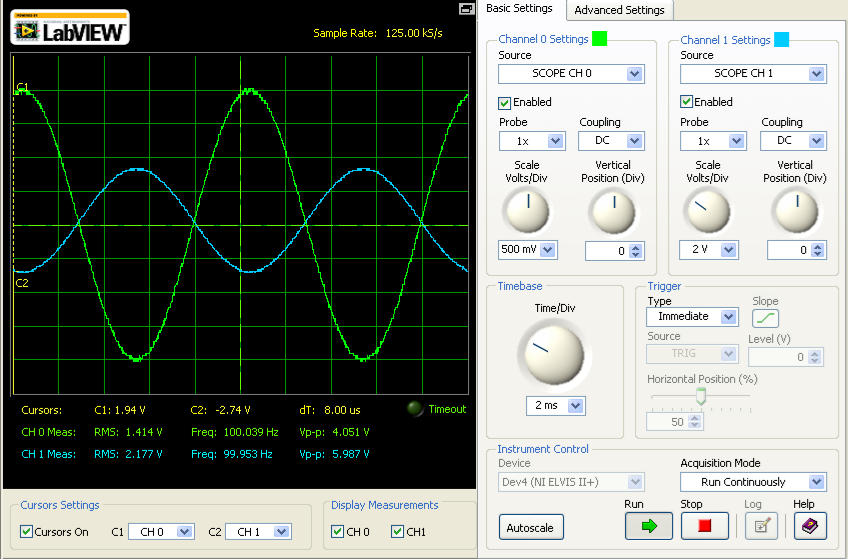
\includegraphics[width=\textwidth]{Imagenes/VBmasVC.png}
		\caption{Sumador en Terminales B y C}
		\label{fig:VBmasVC}
	\end{subfigure}
	\caption{Suma de voltajes}\label{fig:SumadorVoltajes}
	
\end{figure}


\section{Análisis de Resultados}

Logramos verificar el comportamiento de los circuitos planteados experimentalmente a través de verificar sus señales en la salida, además de ver el comportamiento del amplificador operacional como sumador con 3 entradas, la muestra de ello se puede apreciar en la figura \ref{fig:SumadorVoltajes}.\\

\section{Conclusiones}

La Herramienta NI Elvis es de gran utilidad ya que con ella podemos verificar el comportamiento en las salida de un circuito experimental, además de corroborar el correcto funcionamiento del mismo, también podemos obtener la ganancia del circuito y comprobar su función de transferencia.\\

\section{Referencias}

\bibliographystyle{plain}
\bibliography{Referencias.bib}



\end{document}
